\chapter{Approach}
\label{approach}

	Having determined the objectives, the first step of the development process is designing the IDS system's architecture.\ The design involved in this project report is based on the work of Manandhar \cite{Manandhar:TowardsPracticalAnomalyBasedIDS}, which is illustrated in Figure~\ref{fig:originalArchitectureDesign}.
	
	\begin{figure}[hb]
	  \centering
	  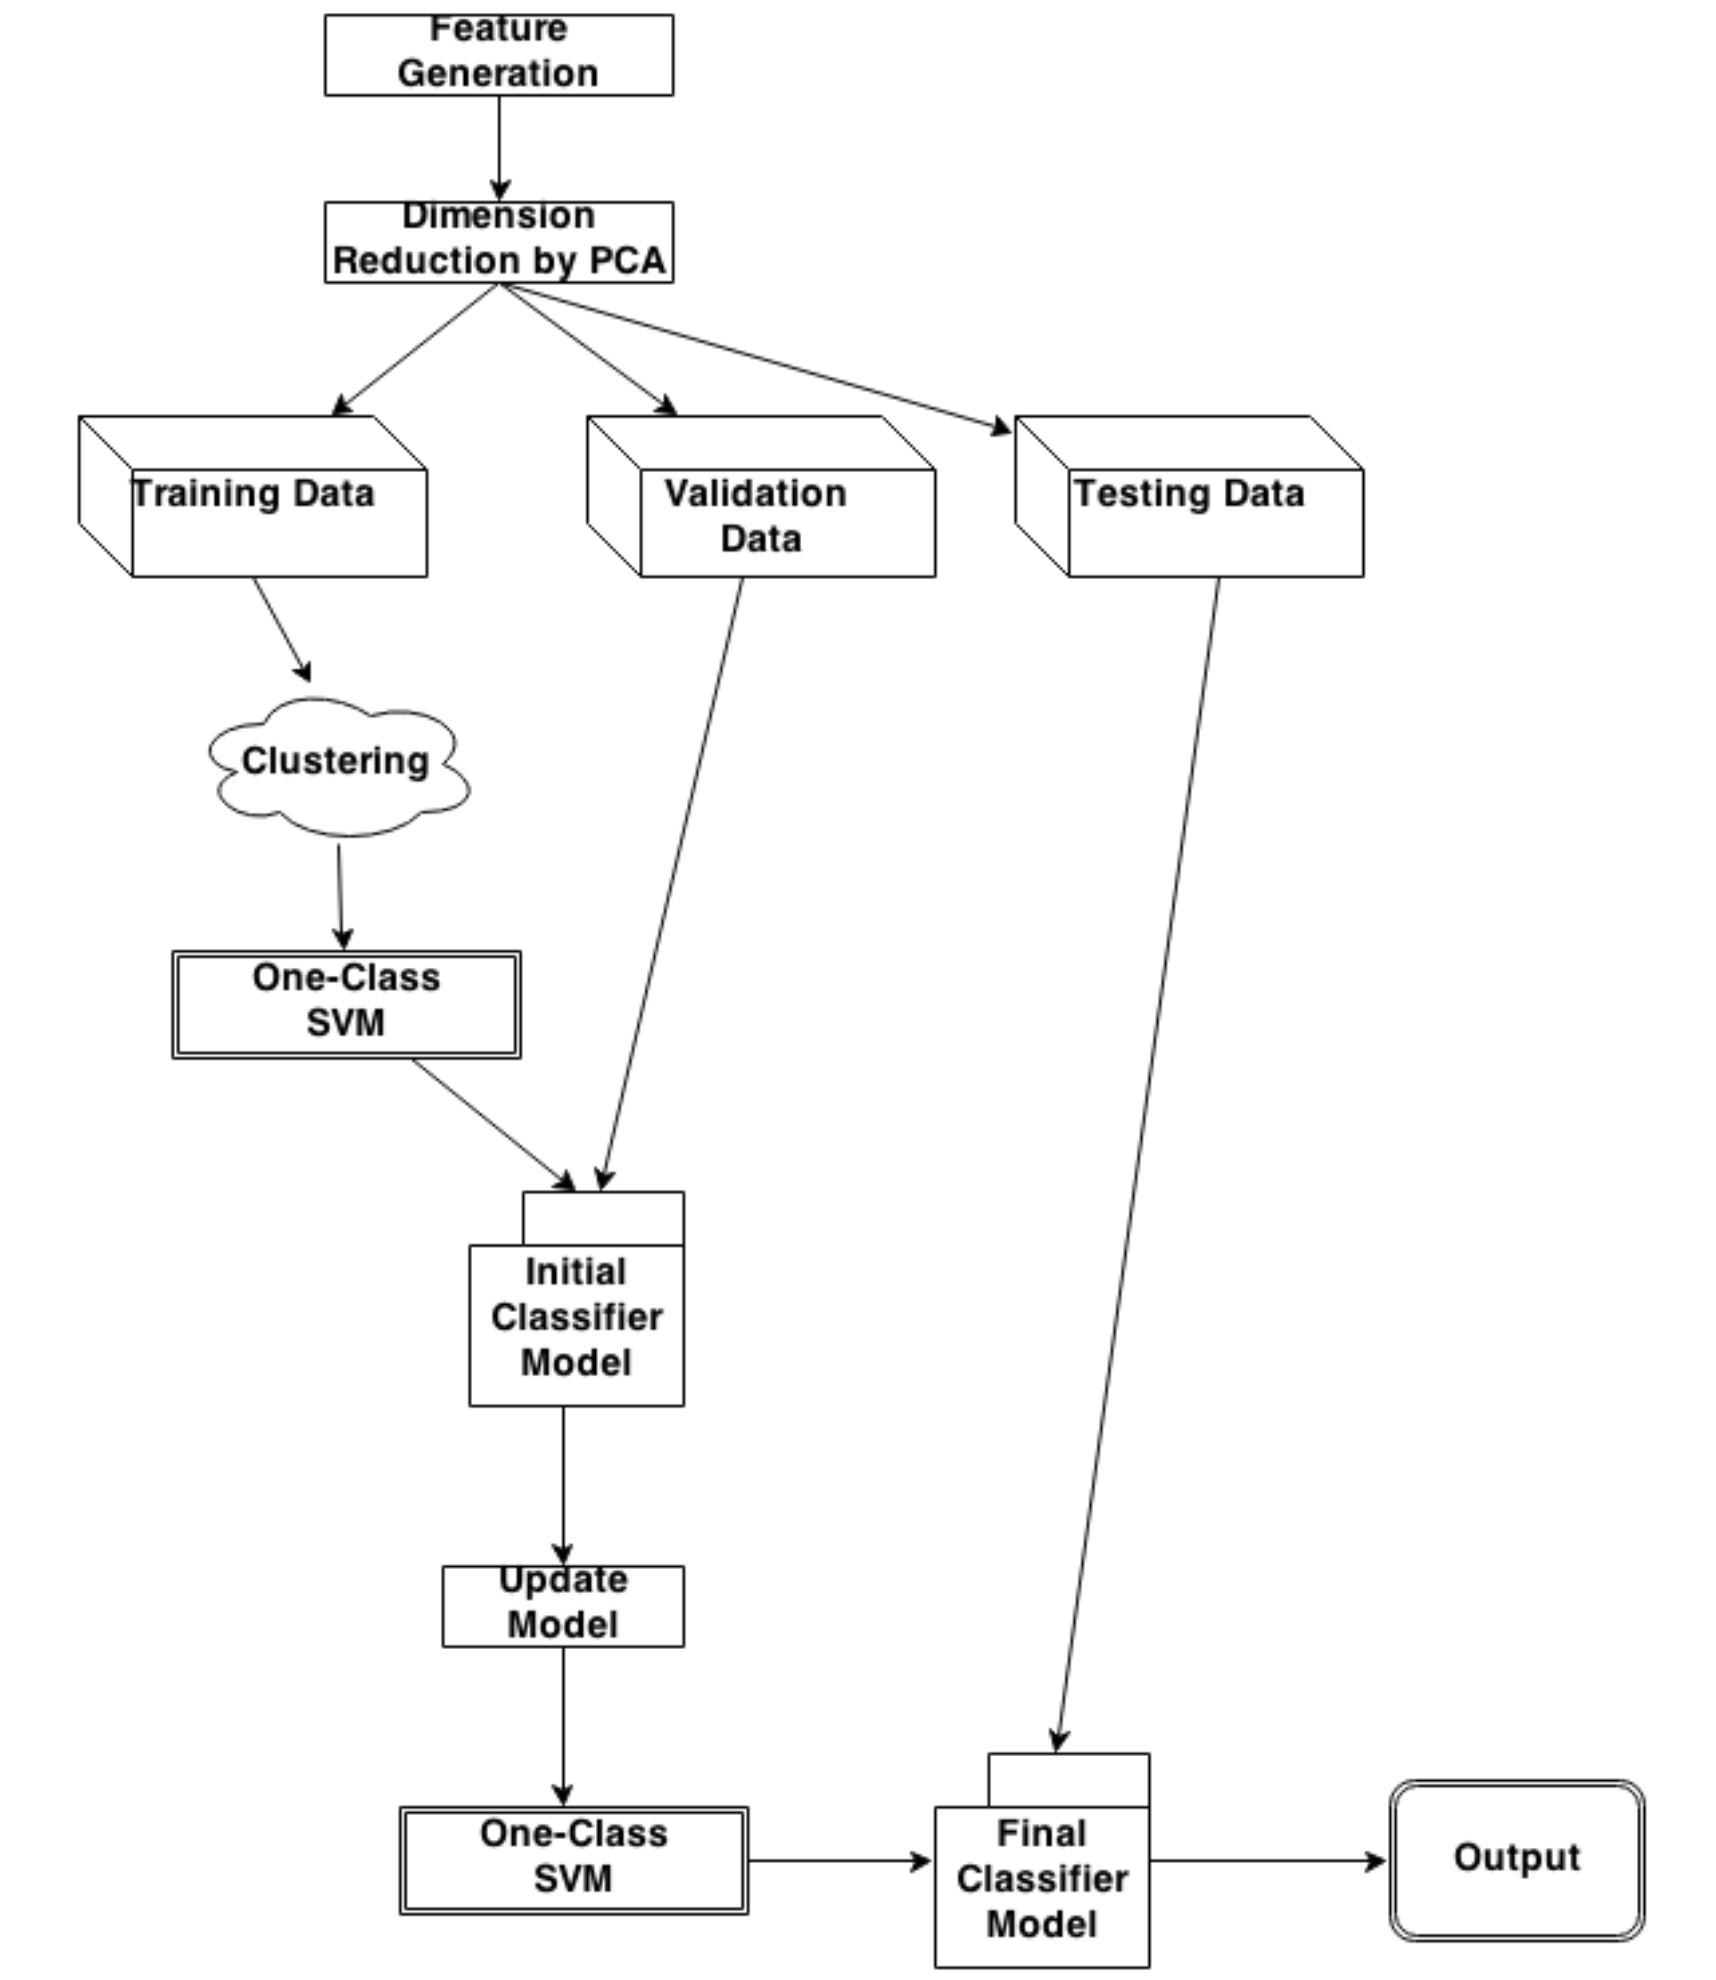
\includegraphics[scale=0.3268]{figures/OriginalArchitecture.png}
	  \caption{Architectural Design of IDS system \cite{Manandhar:TowardsPracticalAnomalyBasedIDS}}
	  \label{fig:originalArchitectureDesign}
	\end{figure}
	
	 The IDS system of this architectural design is set to work on real-time since it performs analysis only based on TCP/IP packet headers.\ The architecture consists of three main components, namely the data-sets preprocessing component, the training component and the testing (classification) component.\ This chapter describes the design of each component and its functionality.
	
	\section{Data-Set Preprocessing Component}

		The data-set preprocessing component is designed to perform extraction of relevant information from given data-sets.\ This component aims to increase the performance of the training component by providing only necessary information that is required to train the IDS system.\ Since the IDS system analyses only TCP/IP packet headers, all packet header information (e.g. payload size, flags, etc.) is extracted from the network packets which is contained in the data-sets. The complete workflow of data-set preprocessing component can be viewed on Figure~\ref{fig:activityDiagramPreprocessing}.

		\begin{figure}[hb]
	 	 \centering
		  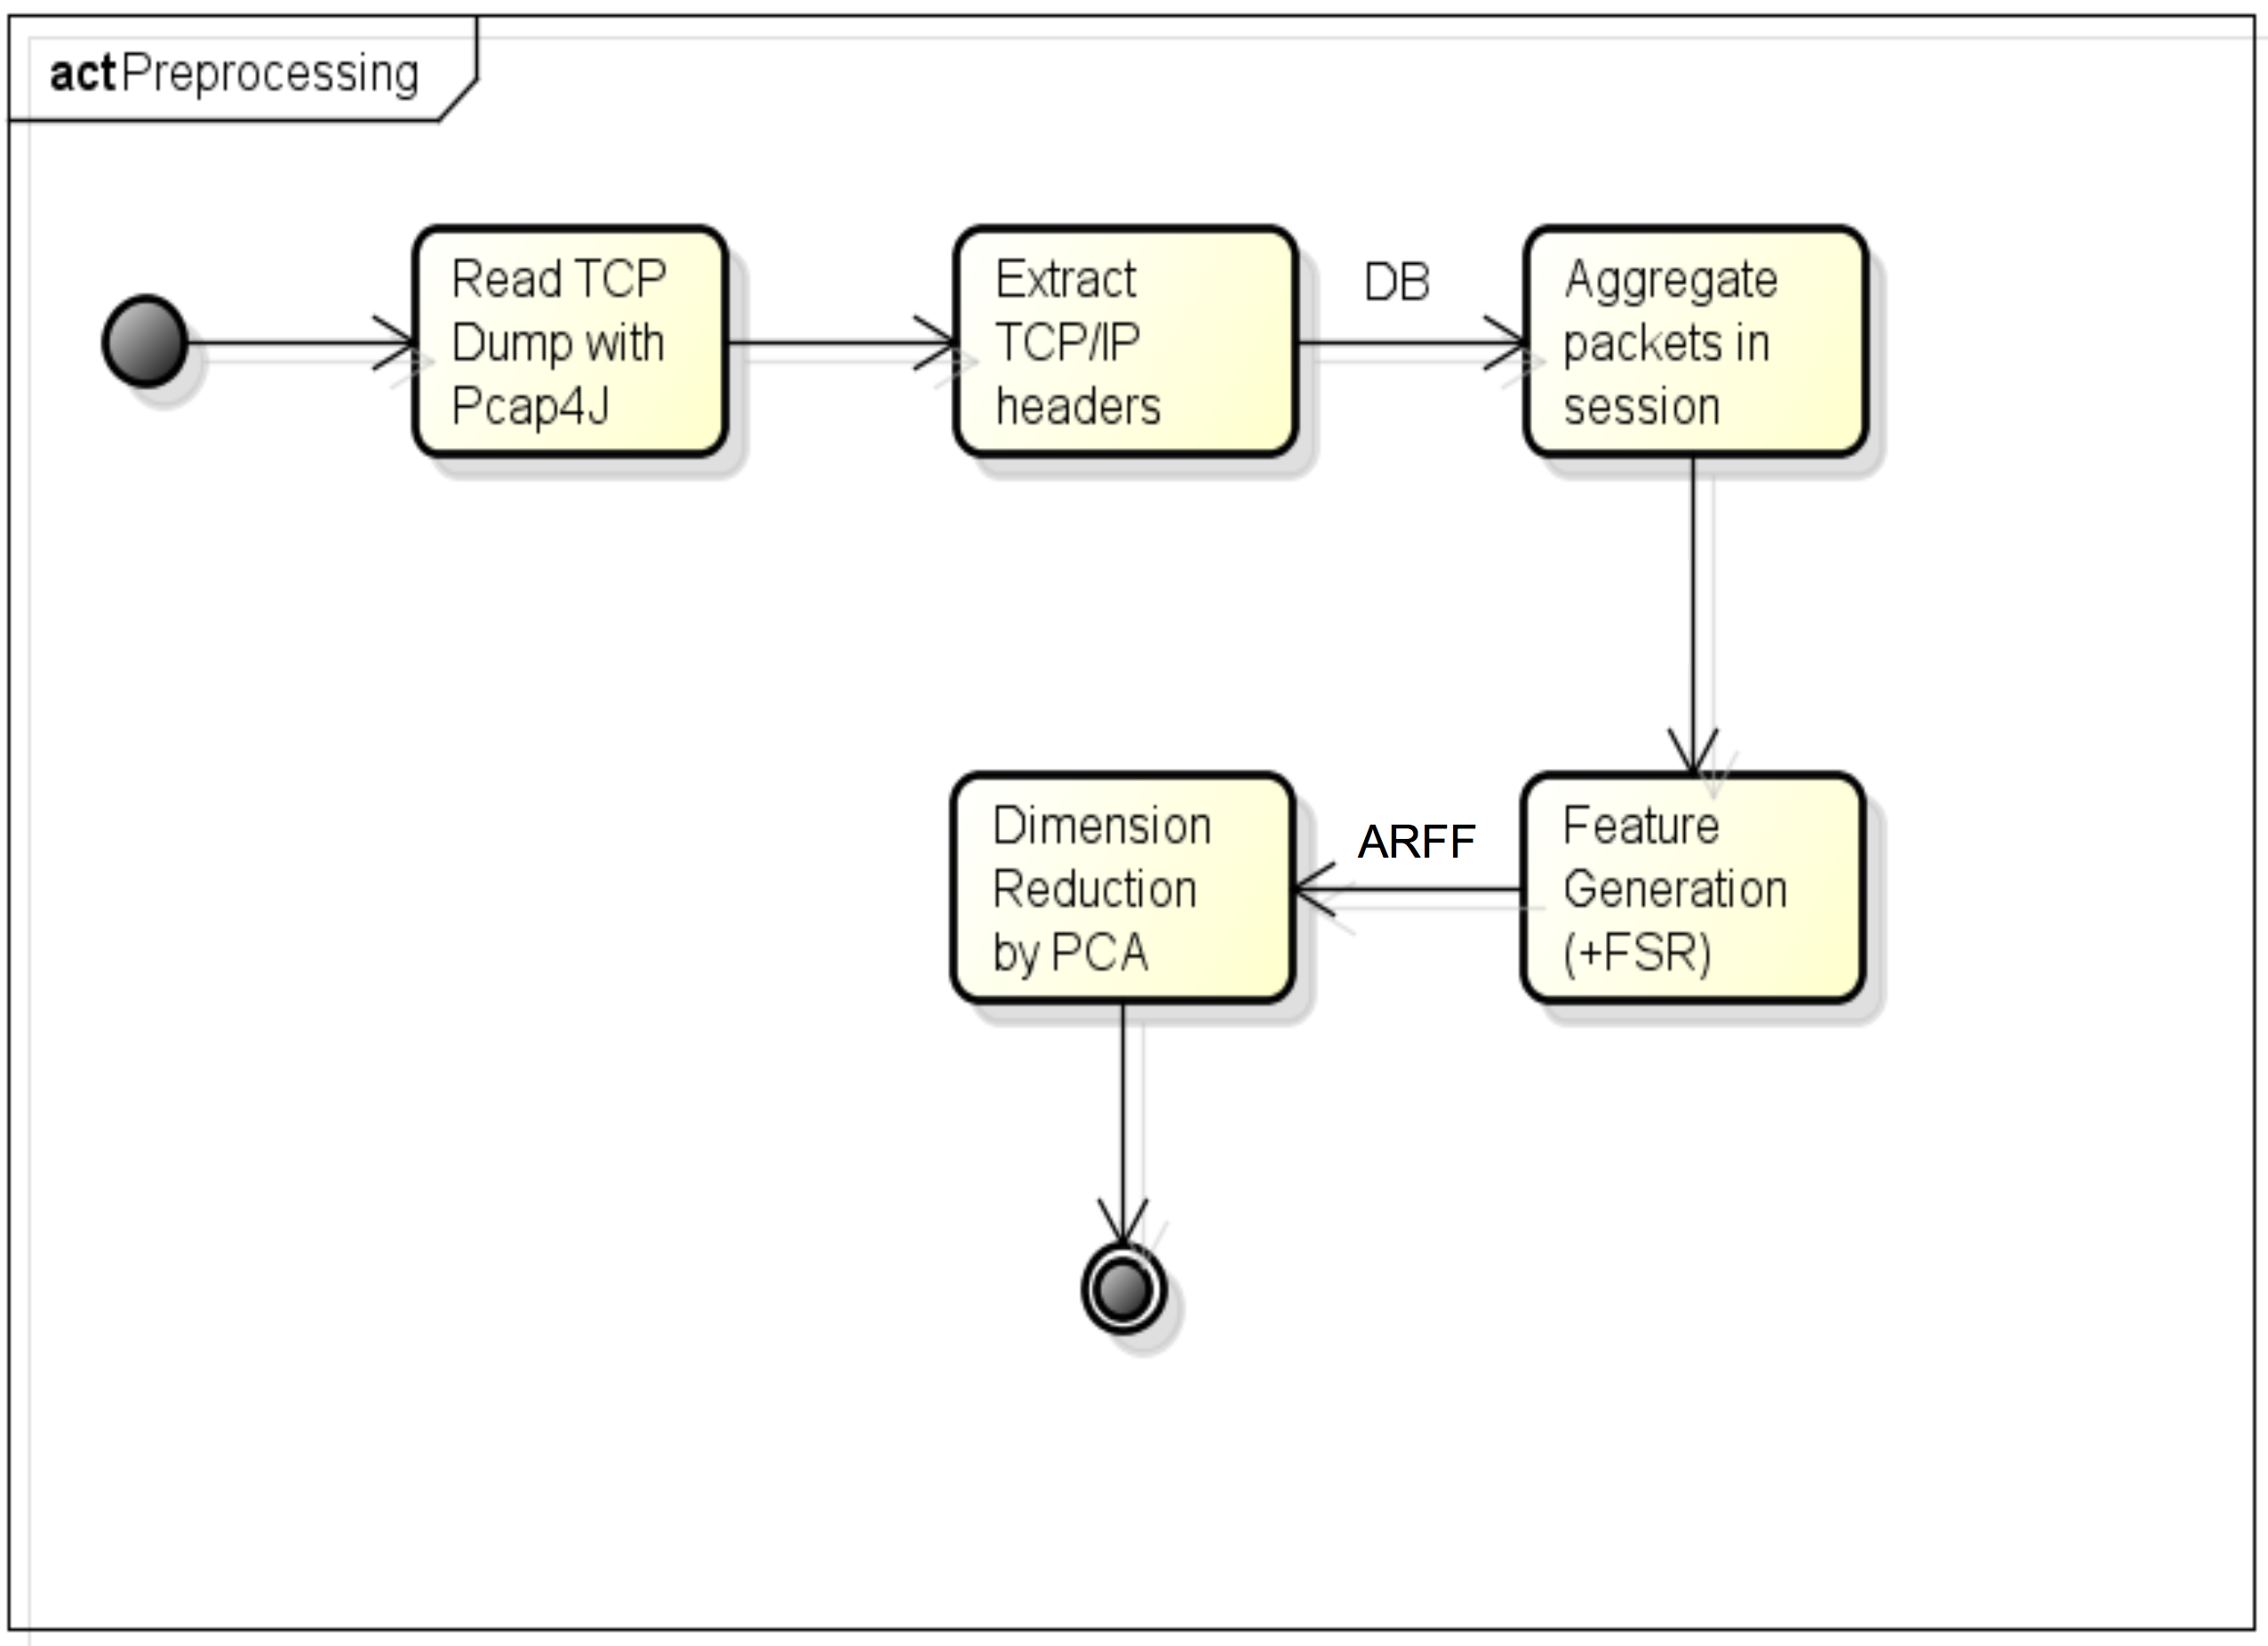
\includegraphics[scale=0.2668]{figures/ActivityDiagramPreprocessing.png}
		  \caption{Activity diagram describing the workflow of data-set preprocessing component}
		  \label{fig:activityDiagramPreprocessing}
		\end{figure}
		
		Preprocessing data-set starts by reading the data-set and converting each network packet into a $Java$ $Object$, which simplifies the header information extraction process.\ Due to the fact that a single abnormal network packet does not provide enough evidence regarding the nature of the network connection, the extracted header information from single packets has to be aggregated to represent one complete network-connection (\textit{TCP-session}).\ The aggregation process is done by building an average of each header information (e.g.\ average payload size, average count of $SYN$-flags, etc.) over four different characteristic of the network packet, namely \textit{source IP-address}, \textit{source port-number}, \textit{destination IP-address} and \textit{destination port-number}.\ This means that all network packets with the same characteristics mentioned above are aggregated into one TCP-session.
		
		Afterwards, the header information is utilised as feature vectors for the training component of the IDS system.\ However, in order to further improve the performance of the training component, the dimensions of these feature vectors are reduced with the help of principal component analysis (PCA).\ The resulting dimensional-reduced feature vectors are then passed onto the training component to be utilised as input for the IDS system's training process. 

	\section{Training Component}
		
		Clustering will be performed on the given dimensional-reduced feature vectors using $k$-$means$ method in order to determine the cluster centroids which serves as input for the one-class support vector machine. The resulting hyper-plane from one-class SVM is the IDS model, based on which the classification component functions.\ A corresponding activity diagram of this workflow is illustrated in Figure~\ref{fig:activityDiagramTraining}.
		
		\begin{figure}[hb]
	 	 \centering
		  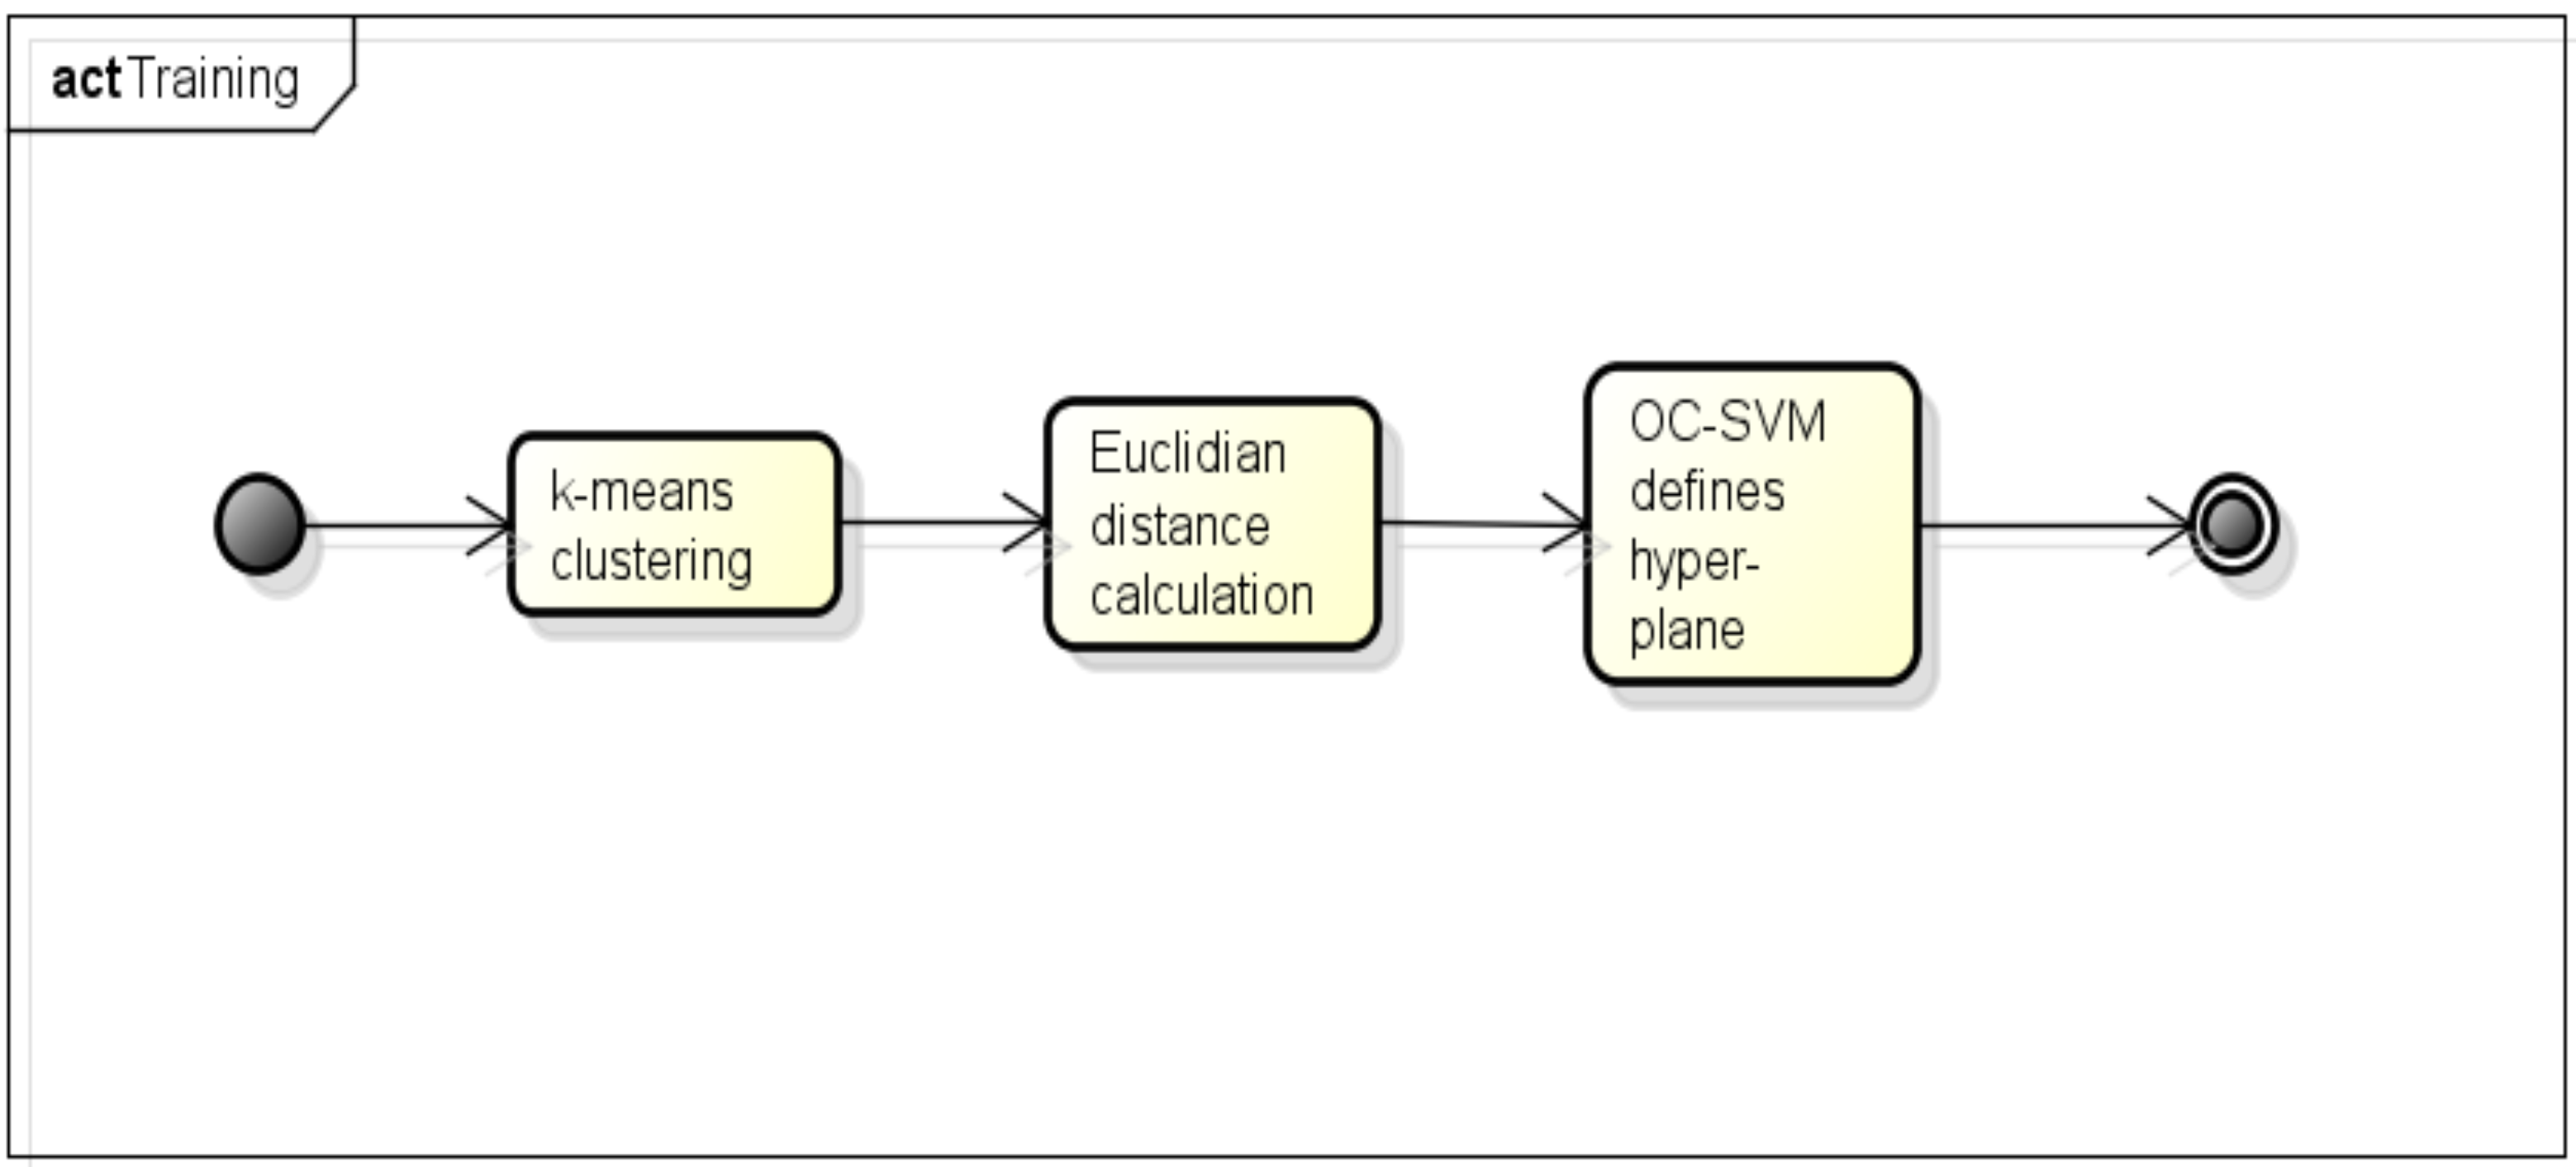
\includegraphics[scale=0.2068]{figures/ActivityDiagramTraining.png}
		  \caption{Activity diagram describing the training process of training component}
		  \label{fig:activityDiagramTraining}
		\end{figure}
				
		Additionally, Manandhar decided on the trade-off between false-positives and false-negatives in the sense that in order to minimise false-negatives, a higher false-positives rate is expected with the design of this IDS system \cite{Manandhar:TowardsPracticalAnomalyBasedIDS}.\ Therefore, the training component is not only responsible for the training process but also for the validation process, whose activity diagram is described in Figure~\ref{fig:activityDiagramValidation}.

		\begin{figure}[hb]
	 	 \centering
		  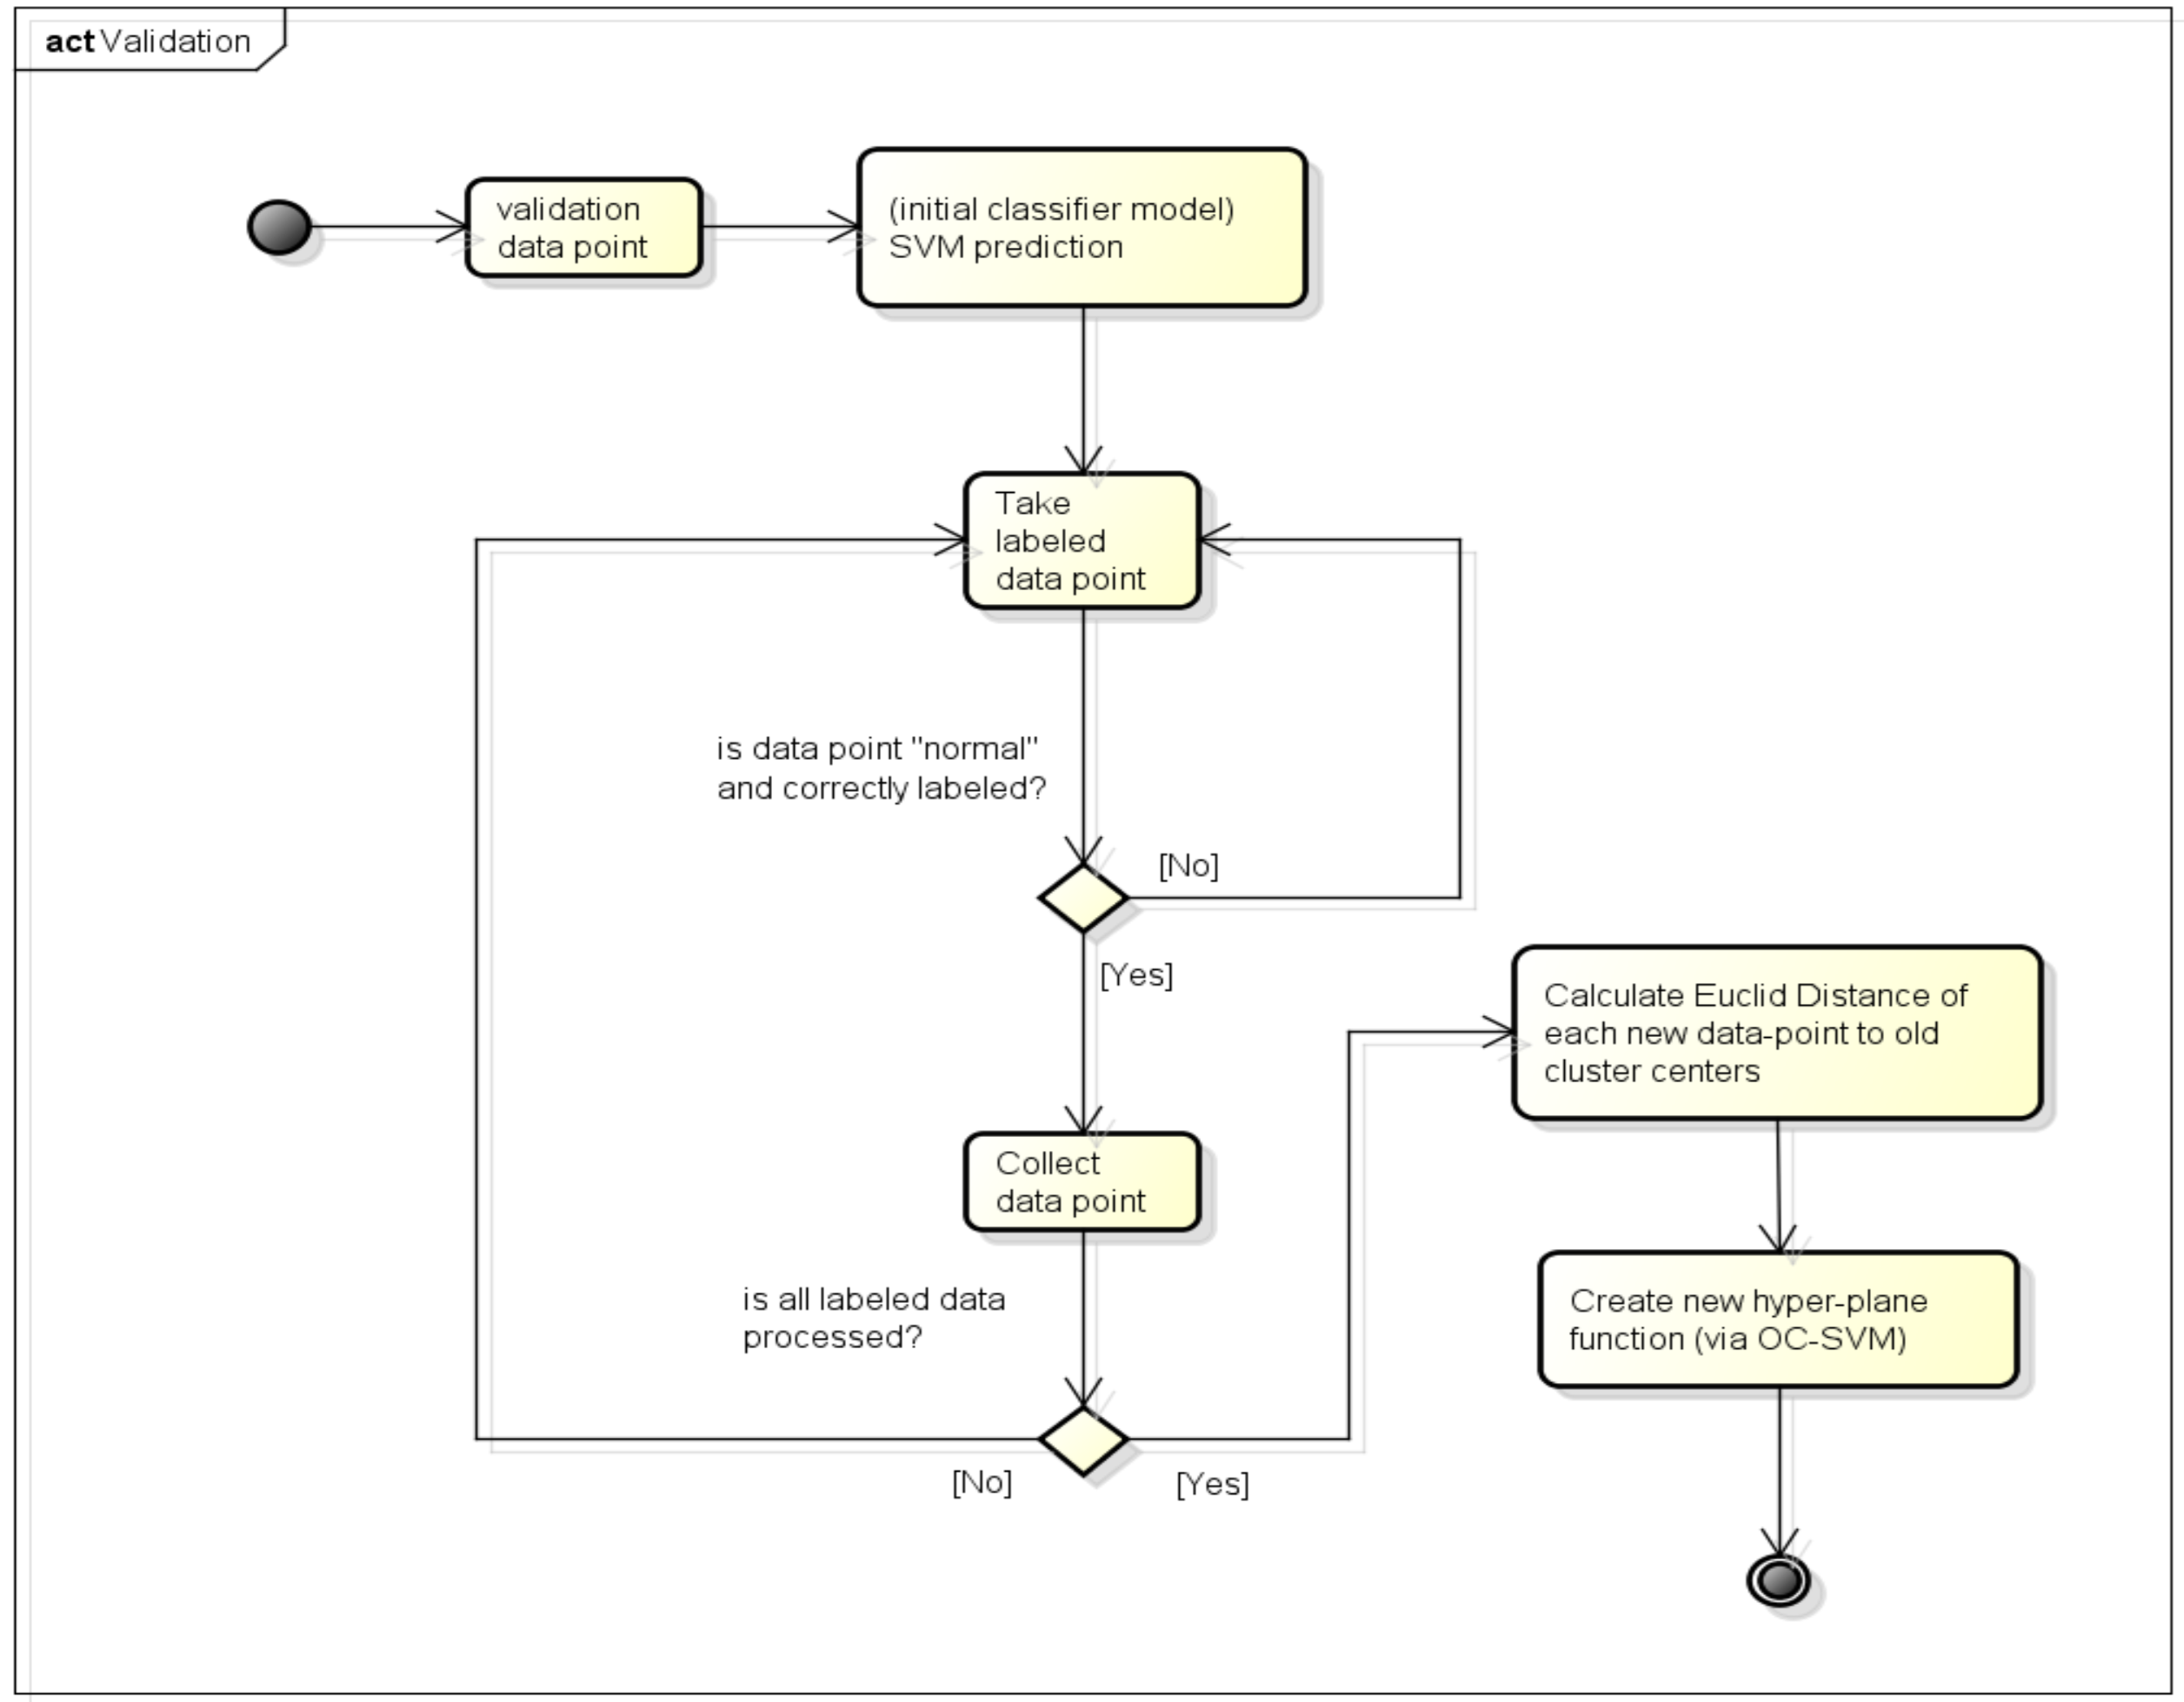
\includegraphics[scale=0.2668]{figures/ActivityDiagramValidation.png}
		  \caption{Activity diagram describing the validation process of training component}
		  \label{fig:activityDiagramValidation}
		\end{figure}
		
		The validation process aims to heightens the sensibility of the IDS detection capability.\ This is achieved by running the classification process on a validation data-set and only 'normal' data-points which were correctly classified by the IDS model (\textit{true positive}) is collected to construct the final IDS model whereas other data-points which were either anomaly or wrongly classified (\textit{true negatives}, \textit{false negatives}, and \textit{false positives}) are ignored and left out.
		
		Data-points collected during the validation process are analysed by calculating the distance of each data-point to all cluster centroids and the distance measure is used as an input for the one-class SVM to construct the final IDS model.

	\section{Classification Component}

		Based on the constructed final IDS model, the one-class SVM is able to classify new data-points.\ Beside the classification result, performance statistics is also collected in order to evaluate the IDS system afterwards.
		


